%# -*- coding: utf-8 -*-
\documentclass{noithesis}

\usepackage[colorlinks,CJKbookmarks=true,bookmarksnumbered,linkcolor=red,citecolor=red,plainpages=true,pdfstartview=FitH]{hyperref}


\begin{document}

\setcounter{page}{129}

%% 论文开始

\title{仙人掌相关算法及其应用}
\author{杭州学军中学\ 王逸松}

\maketitle

\begin{abstract}
近几年来,
信息学竞赛中出现了不少仙人掌相关的问题,
如动态仙人掌问题。
本文将对仙人掌相关的常见算法进行介绍,
并举出一些例题,
希望能起到抛砖引玉的效果。
\end{abstract}





\section{仙人掌的定义和结构}

\subsection{仙人掌的定义}

如果一个无向连通图的任意一条边属于最多一个简单环,且没有自环,我们就称之为仙人掌。

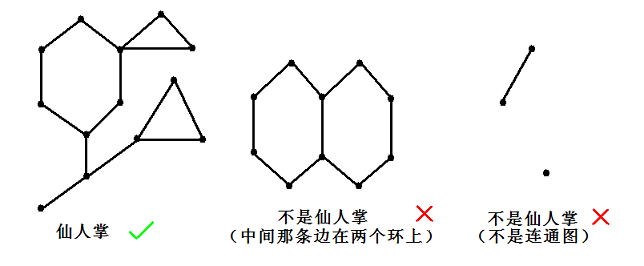
\includegraphics[width=400pt,height=166pt]{images/what-is-cactus.png}

\subsection{仙人掌的边数}

对于一棵$n$个结点的仙人掌,
我们考虑它的一棵生成树,
有$n - 1$条边。
剩下的边均为非树边,每条非树边对应了生成树上的一条路径,并形成了一个简单环。
由于每一条边最多属于一个简单环,任意两条非树边对应的路径的边的交集为空,即这些路径不重叠。
因此最多有$n - 1$条这样的路径,所以$n$个结点的仙人掌最多有$2 n - 2$条边,最少有$n - 1$条边。

\subsection{仙人掌的结构}

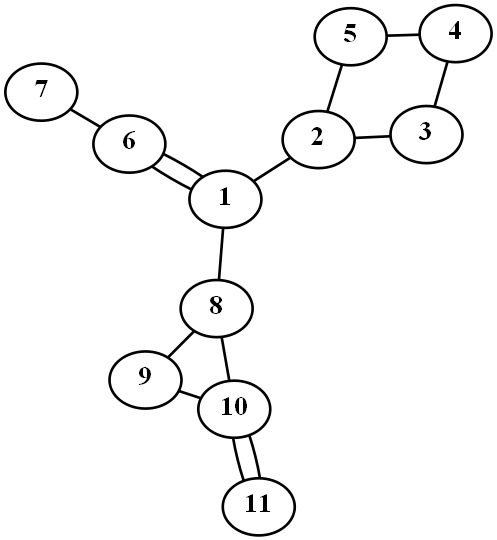
\includegraphics[width=200pt,height=217.3pt]{images/cactus-example.png}

如图是一棵根为1的仙人掌

\subsubsection{父亲}
类比树上结点的父亲,我们定义仙人掌上结点的父亲和环的父亲。

如果一个结点$u$到仙人掌的根之间的所有简单路径的第一条边相同,
那么就类似树上的情况,$u$的父亲为$u$到根的一条简单路径上第二个点,
否则$u$的父亲为$u$到根的一条简单路径上第一条边所在的环。

比如说,8号结点的父亲是1号结点,10号结点的父亲是环8-9-10,11号结点的父亲是环10-11。

一个环的父亲为环上离根最近的结点。

比如说,环8-9-10的父亲为8号结点,环10-11的父亲为10号结点。


\subsubsection{儿子}
类比树上结点的儿子,我们定义仙人掌上结点的儿子和环的儿子。

一个结点的儿子可能是个结点,也可能是个环。

比如说,1号结点的儿子有2号结点、8号结点和环1-6。

一个环的儿子为环上除去环的父亲以外的所有结点。

比如说,环8-9-10的儿子为9号结点和10号结点。


\subsubsection{父亲结点和母亲结点}
对于一个在环上的结点,我们定义它的\textbf{父亲结点}和\textbf{母亲结点}分别为环上与它相邻的两个结点。
(请注意区分\textbf{父亲}和\textbf{父亲结点})

比如说,在环2-3-4-5中,3号结点的父亲结点为2号结点,母亲结点为4号结点,
4号结点的父亲结点为3号结点,母亲节点为5号结点。

从环的任意一个儿子出发,沿着父亲结点和母亲结点就能遍历整个环。


\subsection{如何遍历一棵仙人掌}

类似遍历一棵树的过程,
我们从根开始dfs,
假设当前在结点$x$,接下来要访问结点$y$。

如果$y$还没访问过,
就跟树上的情况一样处理,
只要将$y$的父亲设置为$x$即可。

如果$y$已经访问过,且第一次访问$y$的时间早于第一次访问$x$的时间,
那么说明我们发现了一个环,这个环的父亲为$y$,儿子为$x$到$y$路径上除去$y$的所有点。
我们遍历这个环,并设置环上所有点的父亲结点和母亲结点就行了。

如果$y$已经访问过,且第一次访问$y$的时间晚于第一次访问$x$的时间,
那么说明$y$在一个已经访问过的环上,可以无视这种情况。




\section{仙人掌上的DP}

类比树上的DP,我们可以在仙人掌上进行DP。

从仙人掌的根开始DP,
假设当前DP到结点$u$,
我们先处理结点$u$上的信息,
然后枚举$u$的每一个儿子和以$u$为父亲的每一个环的每个儿子进行DP。

\text{}

\subsection{【例题一】一个经典问题}

给一棵仙人掌,每条边有个长度,求1号结点到每个结点的距离。

其中两个点的距离为它们之间的最短路径的长度。

$n \le 10^5$

\text{}

$\textbf{仙人掌上的DP}$

先dfs一遍仙人掌搞清楚仙人掌的结构。

然后从1号结点开始DP。
假设当前已经求出了1号结点到结点$u$的距离,
我们枚举$u$的每一个儿子,
如果该儿子是一个结点,
那么就能求出1号结点到这个结点的距离,并从这个结点开始继续DP。
否则该儿子是一个环,
我们枚举环上的每个儿子$x$,求出结点$x$到1号结点的距离,然后从$x$开始DP。

时间复杂度是$O(n)$的。

\subsection{【例题二】另一个经典问题}

给一棵仙人掌,每条边有个长度,求直径。

直径的定义是,距离最远的两个点的距离。
其中两个点的距离为它们之间的最短路径的长度。

$n \le 10^5$



\subsubsection{树上的情况}

由于树也是仙人掌,我们先来考虑树上的情况。

一个经典的做法是,随便选一个点,然后找到离它最远的点,
再从这个点开始,再找一次最远的点,这两个点之间的距离即为答案。

\text{}

这个做法在仙人掌上是错的。

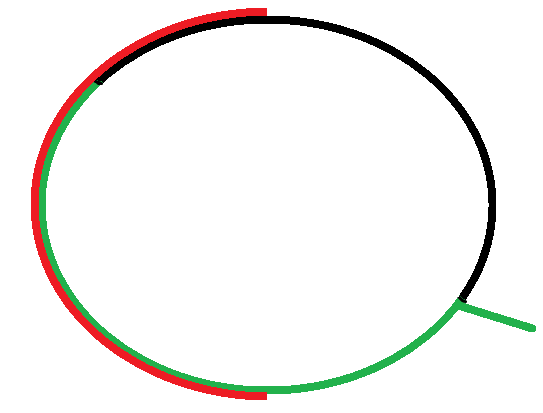
\includegraphics[width=170pt,height=129.7pt]{images/large-cycle-and-one-edge.jpg}

如图,考虑一个有$2 k$个结点的环加上一条边,环上每条边的长度都是1,
那么答案为$k + 1$,但是只有当一开始选到$O(1)$个点时,才能得到这个答案。


\subsubsection{另一种做法}

对于树上的情况,考虑树形DP。
我们可以对每个$x$求出以$x$为根的子树的最大深度,
然后用每个结点的不同儿子的最大深度+次大深度更新答案即可。

对于仙人掌上的情况,可以类比树形DP。
我们先dfs一遍弄清仙人掌的结构,
然后对于每个结点$x$,求出子仙人掌$x$的最大深度。
(子仙人掌$x$的定义是,删掉根到$x$的所有简单路径上的边之后,$x$所在的连通块)

对于每个结点,用它的不同儿子的最大深度+次大深度来更新答案。

对于每个环,还要用环上的每对结点的最大深度的和加上这对结点的最短路长度来更新答案。
不妨枚举其中一个结点,
那么最短路是顺时针走的另一个结点,一定是环上的一个区间,
而且这个区间的另一个端点随着枚举的结点顺时针移动而顺时针移动。
这是个两个端点都单调移动的RMQ问题,可以用单调队列来维护。

也可以不用单调队列。
按照从环的父亲往下走哪边距离近,把环分成两部分。
每一部分内部的点对的最短路一定是在内部走。
对于每个结点,它在另一部分最短路是顺时针走的一定是一个前缀,最短路是逆时针走的是一个后缀,
直接处理前缀max和后缀max即可。

时间复杂度$O(n)$。





\subsection{【例题三】mx的仙人掌 \protect \footnote{Source: \href{http://uoj.ac/problem/87}{UOJ \#87. mx的仙人掌}}}

给一棵n个点的仙人掌和q个询问,
每个询问给定一个点集,要求输出这个点集中距离最远的点对的距离。
两个结点之间的距离为它们的最短路径长度。

$n \le 3 \times 10^5, q \le 3 \times 10^5, $ 点集中点的个数之和$ \mathrm{tot} \le 3 \times 10^5$

时间限制5s,内存限制512MB

\text{}

\textbf{暴力算法}

对每个询问暴力。

对于树上的情况,每个询问只要做一次树形DP即可。

对于仙人掌上的情况,每个询问用上一道例题中的仙人掌上的DP即可。

时间复杂度$O(n q)$。

\text{}

\textbf{一个性质}

在树形DP过程中,如果一个询问给了$cnt$个点,
那么有效的更新答案的次数为$cnt - 1$次,因为一开始有$cnt$个点上有答案,
每次更新答案都会减少一个``有答案''的点。

对于仙人掌上的DP也有类似性质,即有效的更新答案的次数为$O(cnt)$次。

所以对于所有询问,有效的更新答案的次数之和是$O(n)$的。

\text{}

\textbf{树上的情况}

我们可以用$f[x][i]$表示在子树$x$中第$i$个询问的点集中的点到结点$x$的最大距离,
然后树形DP的过程相当于合并这些数组,并更新相应询问的答案。

现在问题转化成,对于每个结点,合并它的每个儿子的DP数组,并快速找到需要被更新答案的询问编号。

这相当于,维护很多数的集合,支持把其中两个合并,
并且在合并的时候返回它们的交集。

可以直接用数组来存集合中的数,然后启发式合并,
即每次合并时,将小的集合暴力插入到大的集合中。
由于要求交集,可以对每个集合开一个哈希表(或直接在全局开哈希表),
然后合并的时候判一下即可。

时间复杂度$O(n \log n)$,空间复杂度$O(n)$。

\text{}

\textbf{仙人掌上的情况}

对于除了环以外的部分,跟树上的情况一样处理。

对于每个环,先将环的每个儿子的DP数组处理出来,
然后用每对DP数组的交集来更新答案。

由于没法从一个集合中删除另一个集合的元素,
所以不能使用带删除操作的单调队列。

可以按照从环的父亲往下走哪边近,将环分成左右两部分,
对环的每一个部分,把DP数组按顺序合并起来,并与另一部分的DP数组求交更新答案即可。

在环上更新完答案后还要撤销所有合并操作,这可以在合并的过程中记录下合并时进行的操作来实现。

最后要把环上所有儿子的DP数组全部合并。

\text{}

\textbf{复杂度分析:}

不考虑环上更新答案时DP数组的合并,总时间复杂度是$O(n \log n)$的,因为每个询问点在合并时作为``较小的集合''最多$O(\log n)$次。

考虑环上更新答案的过程,本质上跟把环上所有DP数组合并是一样的,所以不会影响复杂度,所以总时间复杂度是$O(n \log n)$。

假设环上有若干个集合,总的大小为$N$,那么可以证明,把这些集合按顺序一个一个合并的复杂度不会超过$O(N)$,
所以合并时记录下的操作个数也是$O(N)$,
所以总的空间复杂度也是$O(n)$。

\text{}

\section{仙人掌上的点分治}

类比树上的点分治,我们可以对仙人掌进行点分治。

每次找一个结点(我们称它为``重心''),
使删掉这个结点和这个结点所在的所有环上的边之后,最大的连通块大小最小,
然后统计与重心和重心所在的所有环上的信息,
再递归分治每个剩下的连通块。

\text{}
\newpage

$\textbf{复杂度}$

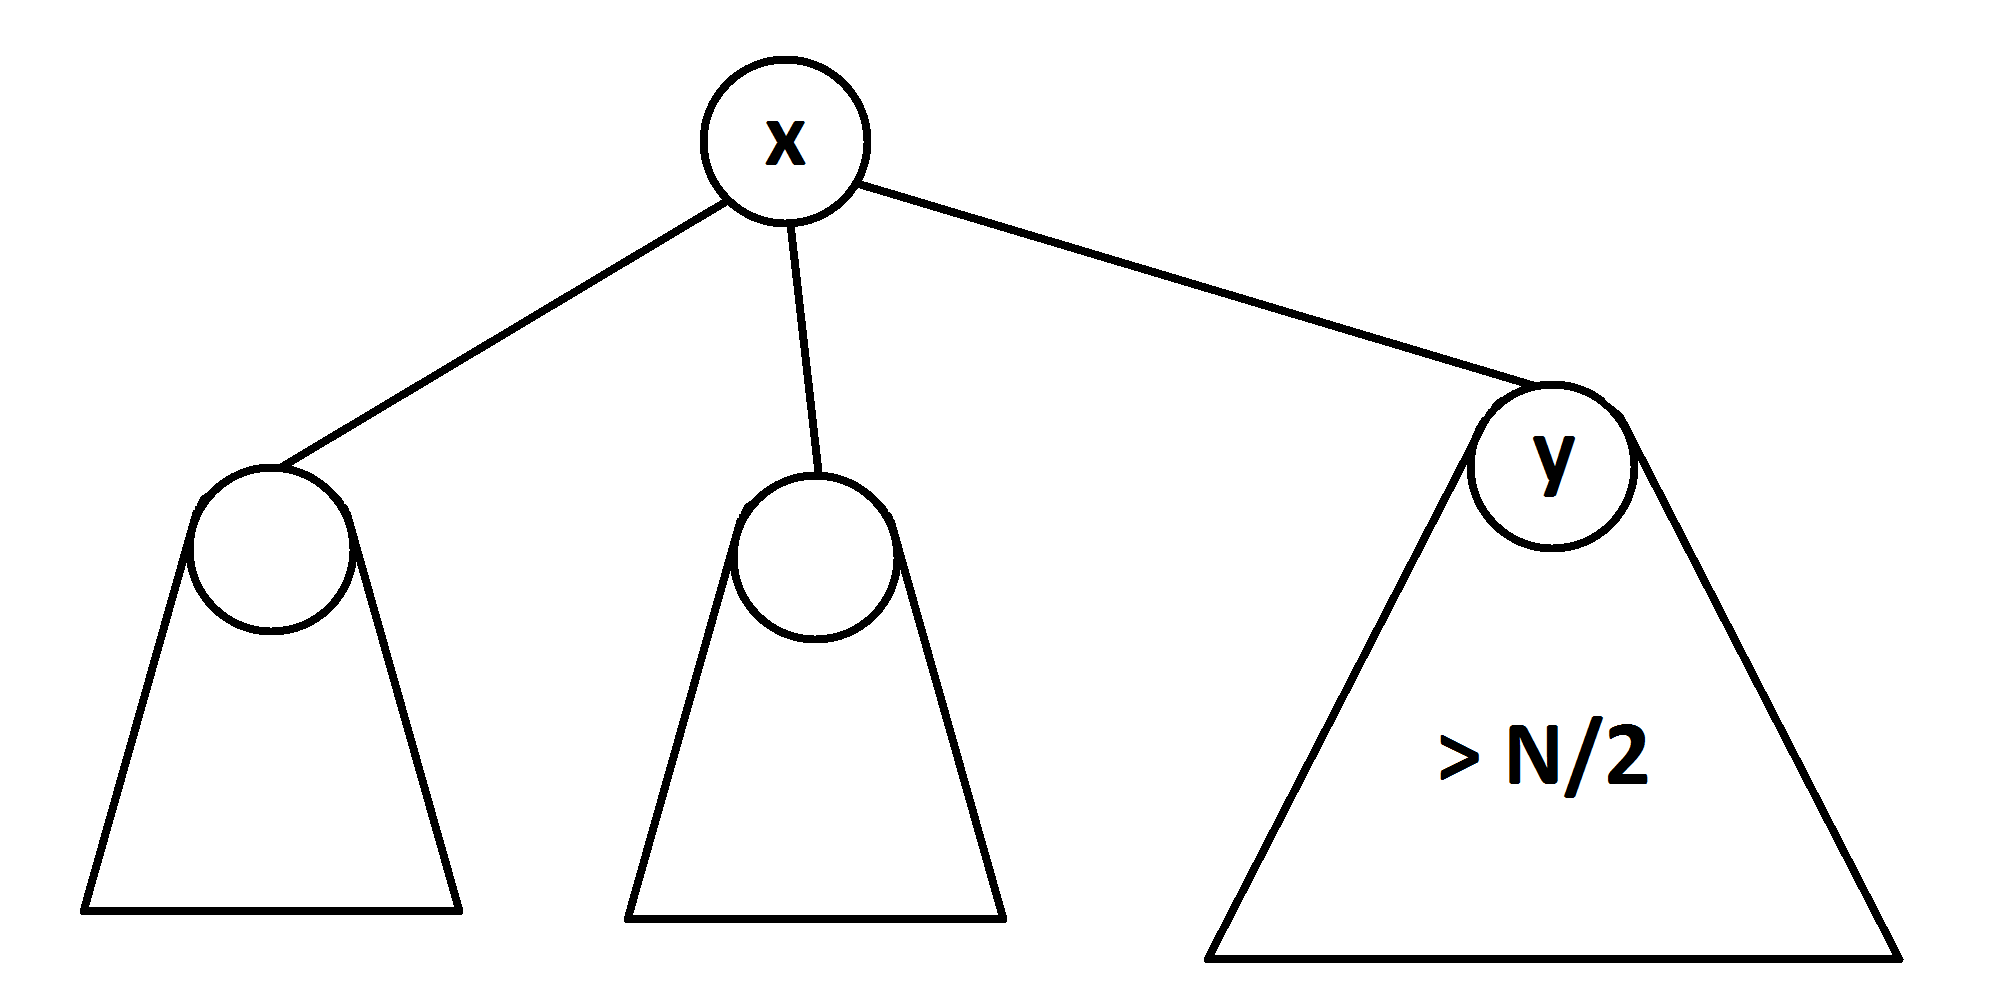
\includegraphics[width=360pt,height=180pt]{images/dac-n-div-2.png}

考虑当前连通块大小为$N$,
如果选择了结点$x$,
并且存在一个结点$y$,使以$x$为根,子仙人掌$y$的大小大于$\dfrac{N}{2}$,
那么选择$y$一定比选择$x$要优。
所以每次分治后,最大的连通块大小至少减少了一半。
所以分治的层数是$O(\log n)$的。

\subsection{【例题一】跳蚤国王下江南\protect\footnote{Source: \href{http://uoj.ac/problem/23}{UOJ \#23. 【UR \#1】跳蚤国王下江南}}}

给一棵仙人掌,求对于$l = 1, 2, \dots, n$,
从1号点出发经过$l$条边的简单路径条数,答案模998244353($7 \times 17 \times 2^{23} + 1$,一个质数)。

$n \le 10^5$

\text{}

\textbf{暴力算法}

记$f[x][l]$为从结点$u$开始,只能向远离根的方向走,长度为$l$的路径条数。

那么对于$x$的每个儿子$y$,
如果$y$是个结点,就把$f[y][l-1]$加到$f[x][l]$里。
如果是个环,那么枚举这个环上的每个儿子$z$,
把$f[z][l-d_1]+f[z][l-d_2]$加到$f[x][l]$里(其中$d_1, d_2$表示$x$到$z$的两条路径的长度)。

\textbf{仙人掌分治}

首先我们发现,$f[u]$可以看作一个多项式,
每次从$u$的一个儿子$v$转移过来时,相当于是把$f[v]$乘上$x$或乘上$x ^ {d_1} + x ^ {d_2}$并加到$f[u]$中。
这启发我们用分治的算法。

对于每次分治,找到重心$u$以后,先递归分治每个连通块,
然后将根到重心的多项式求出来,记为$f(x)$,再将$u$的所有儿子的答案求出来相加,记为$g(x)$。
我们只要将$f(x) \cdot g(x)$和每个连通块的答案加起来即可。

对于求$f(x)$,如果将重心到根的多项式用分治+FFT乘起来,复杂度为$O(n \log ^ 2 n)$。
其实我们可以把递归分治过程中根到重心的多项式记录下来,
然后一个一个乘回去,
复杂度就是$T(n) = T(n/2) + O(n \log n) = O(n \log n)$的了。

总复杂度为$O(n \log ^ 2 n)$。


\subsection{【例题二】Tree and Sets\protect\footnote{Source: 2015年集训队互测}}
有一棵 $n$ 个结点的仙人掌,每条边有一个长度 $l$。(不同的边的长度不一定相同)

有 $q$ 个点集,每个点集可以用两个整数 $u, d$ 来描述($1 \leq u \leq n$),一个结点 $v$ 在这个点集中当且仅当结点 $v$ 与结点 $u$ 的距离不超过 $d$。两个结点之间的距离为它们之间的最短路径的长度。

现在要求构造一个有向无环图(DAG),满足:
\begin{itemize}
\setlength{\parskip}{-7pt}
\item 这个 DAG 至少有 $n+q$ 个结点,至多有 $1200000$ 个结点和 $2400000$ 条边。
\item 对于每一条边,如果是从 $u$ 连向 $v$ 的,那么 $u > n$ 且 $u \neq v$。
\item 对于结点编号在第 $i$ 个点集($1 \leq i \leq q$)的每一个结点 $x$,第 $n+i$ 个结点到第 $x$ 个结点有且仅有一条路径。
\item 对于结点编号在 $\{ 1, 2, \dots, n\}$ 中但不在第 $i$ 个点集($1 \leq i \leq q$)的每一个结点 $x$,不存在第 $n+i$ 个结点到第 $x$ 个结点的路径。
\end{itemize}

$1 \le n, q \le 10000$

\text{}

\textbf{树上的情况}

先给原图加虚点,使每个点的度数都不超过3,
并且对于每个点,要满足最多只有一个点集的$u$为该点。

然后进行树的点分治,每次分治将重心的每一个子树中的所有结点按照到重心的距离排序,
然后预处理前缀和,并对于每个点集连相应的边即可。

由于点分治的层数为$O(\log n)$,所以连边的总数为$O(n \log n)$的。(假设$q = O(n)$)

\text{}

\textbf{仙人掌上的情况}

还是可以先给原图加虚点,使每个点的度数不超过3。
于是这棵仙人掌的每个结点最短属于一个环。

我们可以每次分治找一个结点,或找一个环,
把它作为``重心'',
容易证明这样分治的层数也是$O(\log n)$的。

重心为结点的时候,跟树上的情况一样处理即可。

重心为环的时候,类似仙人掌的DP,将这个环分成两部分,
每一部分之内和两部分之间都是一个前缀和/后缀和的问题。
以每一部分之内的前缀和问题为例,
我们把这一部分当作一个序列,记$size[i]$为序列中下标为$i$的子仙人掌的大小。
每次分治$[l,r]$时,记$\sum_{i=l}^{r} size[i] = N$,
找一个$mid$,使$\sum_{i=l}^{mid-1} size[i] \le N/2$,且$\sum_{i=mid+1}^{r} size[i] \le N/2$,
先递归分治$[l,mid)$和$(mid,r]$,
然后建出$[l,mid)$、$mid$、$(mid,r]$这三部分之间的边。
在这个环上的分治中,对于每个$i$,第$i$棵子仙人掌在$O(\log \dfrac{N}{size[i]}) + O(1)$次分治中出现。
于是对于每个结点,它在每次点分治和每个环上分治的出现次数之和为$O(\log n)$。

所以连边的总数还是$O(n \log n)$的。


\section{link-cut cactus}

\subsection{动态仙人掌问题}

动态仙人掌问题指的是一类在仙人掌上动态维护信息的问题,
动态维护指的可以是修改形态,也可以是修改相关信息。

% \subsection{link-cut cactus}

很多动态树问题可以用link-cut tree解决。
类比link-cut tree,我们能得到link-cut cactus,能用来解决不少动态仙人掌问题。


\text{}

\subsubsection{link-cut cactus的结构}


link-cut tree维护的是树的一个链剖分,
于是我们可以维护仙人掌的一个链剖分。


\newpage

如果没有环,就跟link-cut tree一样,
每个结点有个preferred-child,用实边连起来,
其他儿子用虚边连起来。

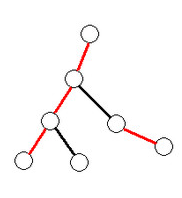
\includegraphics[width=120.33pt,height=132pt]{images/lcc-normal.png}
(红色的边为实边,黑色的边为虚边)

\text{}

对于一个环,我们定义它的父亲为环上离仙人掌的根最近的结点,记为$A$。
我们定义环的preferred-child为环上最后一次access到的结点,记为$B$。

我们将$A$和$B$的最短路用实边连起来。

对于环上其他的结点构成的链,也用实边连起来,我们称这条链为$\textbf{额外链}$(即图中的extra链)。

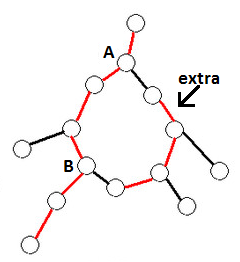
\includegraphics[width=165pt,height=180.125pt]{images/lcc-cycle.png}



\subsubsection{如何在splay上维护边的信息}

在每条边上都加个点,如图所示:

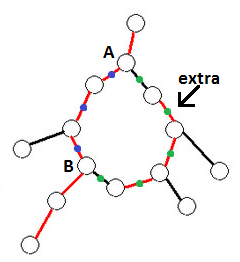
\includegraphics{images/lcc-cycle-1.png}

注意环上额外链两段与$A$和$B$之间的边(黑色边),我们将它直接接在额外链的两端来维护。


\subsubsection{边界情况}

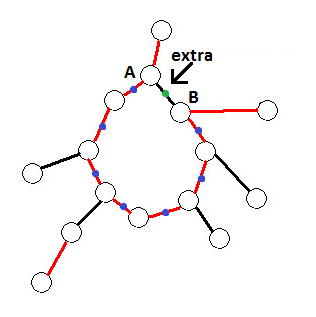
\includegraphics{images/lcc-cycle-2.png}

如图,环上所有的结点都在$A B$链上,于是额外链上只有一条边。
但是我们是在这条边上加了一个点来维护的,所以实际上不需要讨论这种情况。

\subsubsection{一种特殊情况}

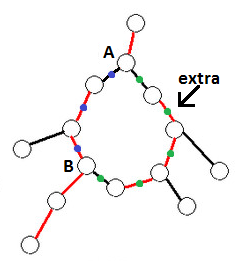
\includegraphics{images/lcc-2b-0.png}

如图,上一次access了结点$A$,这导致了$A B$链上与$A$相连的边变为虚边,
但是表示这条边的splay结点还在$A B$链的splay上。

要注意特判这种情况。




\subsubsection{access操作}

类比link-cut tree的access操作。

假设当前access到结点$x$,
我们先找到$x$在splay上的前一条边$e$。

如果$e$不在环上,
就跟link-cut tree的一样处理。

否则先把这个环的$A B$链的左右两端断开(要注意考虑特殊情况),
然后把$A B$链和额外链连接起来。

然后把$x$提到splay的根,选择较短的一边连回去作为新的$A B$链,
并将另一边设置为额外链。



\subsubsection{换根操作}

类比link-cut tree的换根操作,
在access后对根到该结点的路径打翻转标记来换根。

要注意这会导致这条路径经过的环的$A$和$B$结点互换,而且额外链方向不正确。

解决方法是对于access到的每一个环,检查$A$和$B$在splay中的前后顺序,
如果反了,就交换$A$和$B$,并给额外链打翻转标记。



\subsubsection{如何使用link-cut cactus}

以查询$u$到$v$最短路上边权最小值为例:

先将根换成$u$,然后access结点$v$,
然后返回这棵splay上的边权最小值即可。

要注意$u$到$v$可能有多条最短路,
这个在access到环的时候在splay上打个标记维护即可。


\subsubsection{时间复杂度}

类比link-cut tree,对于$n$个结点的仙人掌和$O(n)$次access操作,
结点和环的preferred-child的切换次数是$O(n \log n)$的,
由于每次preferred-child的切换用到了splay,
所以总时间复杂度为$O(n \log ^ 2 n)$。





\subsection{【例题一】Push\ the\ Flow! \protect \footnote{Source: \href{http://www.codechef.com/problems/PUSHFLOW}{CODECHEF PUSHFLOW}} }

给一棵$n$个点的仙人掌,
保证没有重边或自环,
每条边有个容量。

有$q$个操作,每个操作是修改一条边的容量,或询问两个结点之间的最大流。

$1 \le n \le 100000$

$0 \le q \le 200000$

\text{}

\textbf{link-cut cactus的做法}
\footnote{这题也可以用link-cut tree来解决,由于不是重点略去不讲。}

对于没有环的情况,两个结点之间的最大流就是
这两个结点之间路径上边的容量的最小值。

对于每个环,$A$和$B$结点之间的最大流为$A B$链上的容量最小值加上额外链上的容量最小值,
所以可以将额外链的容量最小值加到$A B$链的每一条边的容量上。

询问时只要换根再access就行了。

修改一条边的容量时,将根换成这条边的一个端点,然后access这条边的另一个端点,
此时需要修改的边一定不会在某个环的额外链上,所以直接修改即可。

时间复杂度$O((n+q) \log ^ 2 n)$,空间复杂度$O(n)$。


\subsection{【例题二】一个经典问题}

给一棵仙人掌,要求支持加边、删边、对某两点之间最短路或某个子仙人掌进行修改或询问。

根为$x$时,子仙人掌$y$的定义是,删掉$x$到$y$的所有简单路径上的边后,$y$所在的连通块。

修改是将一条链或一个子仙人掌的点权加上一个数或修改为同一个数。

询问的是一条链或一个子仙人掌的点权最大值、最小值、和。

\text{}

\subsubsection{一个子问题}

给一棵树,要求支持加边、删边、对某条路径或某个子树进行修改或询问。

\text{}

可以用Self-adjusting top trees来做,时间复杂度为$O(n \log n)$。
这个做法在[\ref{hza}]和[\ref{tarjan_toptree}]中有详细介绍。

\subsubsection{算法一}

我们用link-cut cactus来维护仙人掌的形态。

对于每个环,我们将环上的$B$点与额外链相连的边断开。
(如果这个环上只有两个点,就不把这条边断开)

这样我们就得到了这棵仙人掌的一棵生成树,可以用Self-adjusting top trees(以下简称为``top tree'')维护。

对链进行操作时,在link-cut cactus上换根再access,然后在top tree上进行链操作即可。

对子仙人掌进行操作时,换根再access,然后这棵子仙人掌在top tree上就是一棵子树,直接进行top tree的子树操作即可。

在link-cut cactus的access操作时,会影响到$O(\log n)$个环的preferred-child,
我们要更改那些环上被断开的边,
于是要进行$O(\log n)$次top tree的
link和cut操作,
复杂度是均摊$O(\log ^ 2 n)$的。

由于使用的是top tree,常数有点大。


\subsubsection{算法二}

考虑直接用link-cut cactus来维护。

类比top tree,可以在link-cut cactus的每个结点上维护子仙人掌的信息。
我们将这个做法称为``top cactus''。

$\textbf{一个小技巧}$

我们将需要维护的信息记为$\texttt{Info}$,
标记记为$\texttt{Tag}$,
那么只要实现$\texttt{Info+Info}$,$\texttt{Info*Tag}$,$\texttt{Tag*Tag}$即可。
注意$\texttt{Tag}$可以用a*x+b的形式来表示,可以简化代码。

\text{}

在top cactus的每一个结点上,
我们维护以下几个值:
\begin{itemize}
\setlength{\parskip}{-7pt}
\item $\texttt{x			}$\newline$\texttt{表示该结点本身的信息}$
\item $\texttt{sum			}$\newline$\texttt{表示以该结点为根的splay表示的链上的所有结点的信息和}$\newline$\texttt{(不包含子仙人掌信息)}$
\item $\texttt{sub			}$\newline$\texttt{表示以该结点为根的splay表示的链上的所有结点的子仙人掌信息和}$\newline$\texttt{(不包含链上的信息)}$
\item $\texttt{ex			}$\newline$\texttt{对于每个环的AB链的第一条边,用ex表示该环的额外链的all的值}$
\item $\texttt{all			}$\newline$\texttt{all = sum + sub + ex}$
\item $\texttt{chain\_tag	}$\newline$\texttt{表示对以该结点为根的splay表示的链上的所有结点的标记}$\newline$\texttt{(不包含子仙人掌标记)}$
\item $\texttt{sub\_tag		}$\newline$\texttt{表示对以该结点为根的splay表示的链上的所有结点的子仙人掌的标记}$\newline$\texttt{(不包含链上的标记)}$
\item $\texttt{ex\_tag\_sum	}$\newline$\texttt{表示该环从上次access到以来,AB链上打上的sub\_tag的和}$
\end{itemize}

其中$\texttt{sub}$的值需要枚举每个该结点的每个子仙人掌来求出,
由于一个结点的度数可能为$O(n)$,
所以不能暴力求$\texttt{sub}$,应该对每个结点用一棵平衡树(如splay)来维护$\texttt{sub}$。

$\textbf{标记的下传}$

$\texttt{chain\_tag}$只在splay内部进行下传。

$\texttt{sub\_tag}$下传到子仙人掌时,
被拆成$\texttt{chain\_tag + sub\_tag}$的形式。

$\texttt{ex\_tag\_sum}$维护的是环的$A B$链上已有而额外链上没有的标记,
在access到每一个环的时候下传到该环的额外链上。

$\textbf{access操作}$

每次access到结点$x$时,

如果$x$不在环上:
\begin{itemize}
\setlength{\parskip}{-7pt}
\item 将$x$原来的preferred-child与$x$相连的边改为虚边,并将该preferred-child加入维护子仙人掌的平衡树中。
\item 将$x$的新preferred-child与$x$相连的边改为实边,并将该preferred-child从维护子仙人掌的平衡树中删除,并将子仙人掌标记传给它。
\end{itemize}

如果$x$在环上:
\begin{itemize}
\setlength{\parskip}{-7pt}
\item 将环的上下两端断开,找到$A B$链上的$\texttt{ex\_tag\_sum}$,将其传给额外链。
\item 将$x$提到splay的根,选择较短的一边接回去,并更新相应的信息和标记。
\end{itemize}


$\textbf{时间复杂度}$

link-cut cactus本身的复杂度为$O(n \log ^ 2 n)$。

access循环的总次数为$O(n \log n)$,
所以维护每个结点的子仙人掌信息的复杂度也是$O(n \log ^ 2 n)$。

总时间复杂度为$O(n \log ^ 2 n)$,但是常数比上一个算法要小。






\subsection{【例题三】一个经典问题\ EXT}

给一棵仙人掌,要求支持加边、删边、对某两点之间最短路或某个子仙人掌进行修改或询问。

根为$x$时,子仙人掌$y$的定义是,删掉$x$到$y$的所有简单路径上的边后,$y$所在的连通块。

修改是将一条链或一个子仙人掌的点权加上一个数或修改为同一个数。

询问的是一条链或一个子仙人掌的\textbf{第$k$大}点权。

\text{}

\subsubsection{一个子问题}

给一棵树,要求支持加边、删边、对某条路径或某个子树进行修改或询问第$k$大点权

\text{}

top tree并不能用来维护第$k$大。

我们考虑维护链和子树信息的另一种经典做法:dfs序

由于有链修改和询问第$k$大,维护dfs序的数据结构可以是块状链表。

假设块状链表的块大小为$T$,那么在块状链表上一次分裂或合并操作需要$O(\log n + T)$的时间,
一次询问操作需要$O(\dfrac{n}{T} \log ^ 2 n)$的时间。
(注意可以用平衡树来维护块的序列,就能做到$O(\log n +T)$的修改复杂度)

如果我们能将原问题的每个操作转化成$f(n)$个dfs序的分裂、合并操作和$O(1)$个询问操作,
那么将块状链表的每块大小设为$O(\sqrt{\dfrac{n \log ^ 2 n}{f(n)}})$,
每个操作的时间复杂度就是$O(\sqrt{n f(n) \log ^ 2 n})$。

\text{}

\textbf{树的形态不变,且树根固定}

我们用link-cut tree来维护这棵树的一个链剖分,
然后维护一个对应的dfs序列。

在这个dfs序列上,所有链剖分里的链在dfs序上都是一段区间。

我们在link-cut tree的access过程中对dfs序列进行相应的调整。

假设当前要将结点$x$的preferred-child改为$y$,
就只要把子树$y$所对应的dfs序列的区间取出来,放到结点$x$后面。

这样在access了结点$x$之后,根到$x$这条链在dfs序上是个区间,
子树$x$在dfs序上也是个区间,于是就能进行链和子树操作了。

\text{}

\textbf{树的形态不变,有换根操作}

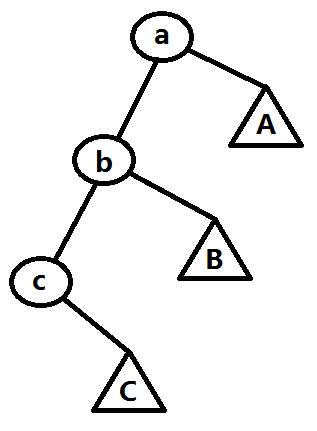
\includegraphics[width=120pt,height=163.1pt]{images/tree-abc.png}

图中椭圆表示结点,三角形表示子树。

根为$a$时,这棵树的dfs序列为$a\ b\ c\ C\ B\ A$。(小写字母表示结点,大写字母表示子树)

根为$c$时,这棵树的dfs序列为$c\ b\ a\ A\ B\ C$。

假设我们要把根从$a$换到$c$。

首先access新根,进行了$O(f(n))$次dfs序操作。

然后只能用$O($树高$)$次dfs序操作来换根?

\text{}

\text{}

不妨强行对原根到新根这条链所在的dfs序区间和dfs序剩下的部分打翻转标记。

这样dfs序列就变成$c\ b\ a\ r(A)\ r(B)\ r(C)$了。($r(X)$表示将$X$这棵子树的dfs序翻转后得到的序列)

注意某些子树的整个dfs序列都反了。

我们在access的每一次循环中,检查一下是否发生了这种情况,
如果有的话,就用$O(1)$次dfs序的操作把这个子树的dfs序列翻转回去。

这样就能做到$f(n) = O(\log n)$了。

\text{}

\newpage

\textbf{树的形态可以改变}

对于加边和删边操作,
我们在换根、access相应的结点后,
直接将整棵树的dfs序列接上去或分离出来即可。

仍然满足$f(n) = O(\log n)$。

\text{}

于是对于这个子问题,我们能做到每个操作$O(\sqrt{n \log ^ 3 n})$的复杂度。

\subsubsection{仙人掌上的情况}

我们还是用link-cut cactus来维护仙人掌的形态,
一次操作可以转化成$O(\log n)$次树上的问题的操作。
于是我们得到了$f(n)$的上界,为$O(\log ^ 2 n)$。
但是写个程序后会发现,$f(n)$更接近$O(\log n)$。

下面给出$f(n) = O(\log n)$的证明:

因为link-cut tree维护的是仙人掌的生成树,且维护时access到的点一样,
于是在LCT上的链剖分与link-cut cactus维护的链剖分类似,
那么在一次link-cut cactus的access中,
除了LCT的第一次access以外,
每一次LCT的access都只改变了1个环的链剖分,经过了$O(1)$条虚边,
这就说明了,LCT的access循环总次数是$O(\log n)$,
所以$f(n) = O(\log n)$,

于是这题就在每个操作$O(\sqrt{n \log ^ 3 n})$的复杂度内解决了。



\section{感谢}

感谢CCF提供的学习交流的机会。

感谢教练徐先友对我的培养。

感谢帮助我完成论文的同学们。


\section*{参考文献}
\begin{enumerate}[\lbrack 1\rbrack]
\item \label{hza} 黄志翱, 浅谈动态树的相关问题及简单拓展, 2014年国家集训队论文
\item \label{tarjan_toptree} Tarjan, Robert E., and Renato F. Werneck. ``Self-adjusting top trees.''
\end{enumerate}











% \section{论文要求}

% 第一节的正文内容。

% \subsection{小节标题}

% 小节的正文内容。

% 公式:
% \begin{eqnarray}
% \left(a+b\right)^2&=&a^2+2ab+b^2 \label{eq:sqr},\\
% \frac{1}{x(x+1)}&=&\frac{1}{x}-\frac{1}{x+1}.
% \end{eqnarray}

% 由(\ref{eq:sqr})可知,$a^2+b^2\geq 2ab$。

% \subsubsection{小小节标题}

% 小小节的正文内容。

% \subsection{小节标题}

% 小节的正文内容。

% \subsubsection{小小节标题}

% 小小节的正文内容。

% \subsubsection{小小节标题}

% 小小节的正文内容。



% \section*{参考文献}
% \begin{enumerate}[\lbrack 1\rbrack]
% \item Mokhtar S. Bazaraa, John J. Jarvis, and Hanif D. Sherali, ``Linear Programming and Network Flows (4th ed.)'', John Wiley \& Sons Inc.
% \item 刘汝佳, 黄亮, 《算法艺术与信息学竞赛》, 清华大学出版社。
% \item 刘汝佳, 《算法竞赛入门经典》, 清华大学出版社。
% \end{enumerate}

%% 论文结束

\end{document}
